\section{はじめに}
\label{sec:hajimeni}
\subsection{社会的背景・課題・本稿の目的}

近年，動画配信サイトやストリーミングサービスの普及によって，誰もが手軽に音楽コンテンツを視聴できる環境が整っている．特に日本では，ゲームやアニメなどのサブカルチャーを起点とした音楽コンテンツが数多く生み出されており，独自の文化として定着している．
一方で，このようなデジタル配信の消費形態は，実際に会場へ足を運んで演奏を体感するライブイベントやコンサートとの相乗効果を生み，市場規模の拡大にも寄与している\cite{cul}\cite{live}．たとえば，博報堂の谷口による分析では，ストリーミングサービスの利用者がサービス内で新たに好みのアーティストを複数発掘し，そのアーティストたちを一度に鑑賞できるライブやフェスへ参加するという行動の流れが形成されつつあり，さらにライブでの体験を通じて別のアーティストと出会うことで，再びストリーミングでの視聴に戻るという音楽消費サイクルが生まれていると指摘されている\cite{taniguchi2019}．すなわち，デジタル配信とライブイベントは互いの顧客を送客し合う関係にあり，この循環が音楽市場全体の拡大を後押ししていると考えられる．実際に，一般社団法人コンサートプロモーターズ協会が実施したライブ市場調査によれば，2025年におけるライブ市場の年間売上高は6443億円，入場者数は5999万人にのぼり，デジタル配信の普及以降もライブ市場は堅調に拡大を続けている\cite{acpc}．図\ref{fig:live_market}に示すように，国内のライブ・コンサート市場における年間売上額は2010年の1280億円から2019年の3665億円まで，10年間でおよそ2.9倍に拡大している．2020年には新型コロナウイルス感染症の影響により，会場に人を集めること自体が困難となった結果，年間売上額は779億円まで急落した．しかし，行動制限の緩和とともに市場は急速に回復し，2022年には3984億円，2023年には5140億円，そして2025年には過去最高となる6443億円を記録している．この推移から，ライブ会場に足を運ぶという体験に対する需要は，一時的な外的要因によって落ち込むことはあっても，長期的には一貫して拡大する傾向にあると言える．

\begin{figure}[tb]
  \centering
  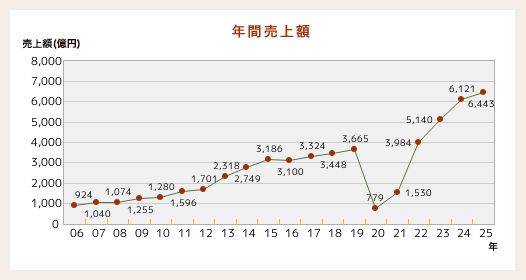
\includegraphics[width=0.7\linewidth]{figs/acpc_sales_transition.png}
  \caption{国内ライブ・コンサート市場における年間売上額の推移（一般社団法人コンサートプロモーターズ協会「基礎調査推移表」より)}
  \label{fig:live_market}
\end{figure}

デジタル配信が普及していく中で，なぜデジタル配信では代替できない価値がライブ会場に存在するのだろうか．その理由の一つとして，ライブ演出に用いられる音響や照明，ライブ参加者自身が感じる振動といった複数の物理的刺激が挙げられる．これらの刺激は，観客一人ひとりに個別に届けられるのではなく，同じ空間にいる観客全員に同時に共有されるという性質を持つ．その結果，観客同士が同じ体験を共有しているという感覚，すなわち空間全体としての一体感が形成される．換言すれば，ライブ会場における没入感とは，ユーザが音楽を聴くだけでとどまらない，物理的，視覚的な技術を同じ空間で同時に受け取ることによって生まれる体験だと考えられる．
この仮説は，複数の研究によっても裏付けられている．ライブ演奏とデジタル配信を直接比較した実証研究によっても裏付けられている．
Kreuzerら（2025）は，同一のクラシック音楽コンサートを，会場で聴取する条件と映像配信で視聴する条件とで比較する実験を行った．その結果，没入感や社会的なつながりの感覚を含む複数の評価軸において，ライブ条件の方が配信条件よりも有意に高い評価を得ることを示した\cite{Kreuzer2025}．すなわち，同じ演奏内容・同じ音質であっても，同じ空間を他の観客と共有しているという感覚そのものが，没入感を左右する独立した要因であり，これは録画・配信技術の高度化だけでは補えないことを意味する．したがって，音そのものの再現性だけでなく，ライブ体験に固有の空間的フィードバックを組み込むことで没入感の高い演奏体験の実現に有効であると考える．

また，Natalia Cooperら（2018）は，仮想現実（VR）環境における体験の再現度を高めるため，視覚情報のみでは表現が難しい感覚を，音や触覚など別の感覚を用いた代替フィードバックとして提示する実験を行った．その結果，視覚刺激のみを提示した場合と比較して，音や触覚といった複数の異なる刺激を組み合わせて提示した場合の方が，利用者の没入感・関与感が有意に高まることを明らかにした\cite{Natalia2018}．つまり，複数の感覚情報を同時に提示する多感覚的フィードバックは，ユーザの体験における没入感の向上に有効であると考える．また，Human-Computer Interaction（HCI）分野の知見も同様の傾向を支持している．Martinら（2024）は，ライブコンサート環境を対象とした研究において，観客が演奏を受動的に聴取するだけでなく，能動的に体験へ参加することが，会場全体の活気や観客の感情の高まりに寄与すると結論づけた\cite{Martin}．よって，ユーザ自身が能動的に関与できる仕組みもまた，システムの没入感を高める要因として重要であると考える．

一方，音楽を自動で演奏する自動演奏技術の分野では，デジタル技術の発展により高精度な同期や楽曲再現が可能になっている．たとえば，Yamahaが提供するDisklavier ENSPIREシリーズは，光学センサとサーボモータを用いて演奏情報を高精度に再現するとともに，鍵盤が実際に動作する様子をユーザへ視覚的にフィードバックを行う機能を備えている\cite{yamaha}．しかし，この視覚的フィードバックは，ピアノの鍵盤という限られた範囲でのみ提示されるものであり，その場に居合わせたユーザ１人のみが確認できる情報にとどまる．したがって，複数人が同じ空間にいる状況を想定すると，自動演奏技術によって提示される視覚的フィードバックは，空間全体には行き渡らないという限界を抱えていると言える．

以上を踏まえると，現状の自動演奏技術は，演奏そのものの精度は高い一方で，前述した「多感覚的フィードバック」と「空間全体への共有」という，没入感を高めるうえで重要な要素を十分には満たせていないという課題が生じる．特に，Kreuzerらの知見が示すとおり，同じ場を共有しているという空間的なフィードバックは，音質や演奏精度をいくら高めても代替できない，ライブ体験に固有の要素である．したがって，デジタル配信や高精度な自動演奏技術がどれほど発展しても，この空間的フィードバックを欠いたままでは，ライブ会場に匹敵する高い没入感を得ることはできないと結論づけられる．そこで本稿では，自動演奏技術に，ライブ体験に共通するこの空間的フィードバックを付加した楽器間通信システム「回転機構のレーザー受光と楽器間無線通信による同期・輪唱システム」を提案する．本システムは，ユーザの動作を検知する指揮デバイス，指揮デバイスからの情報に応じ回転する観覧車型の中継機デバイス，そして中継機からのレーザー光を受光し演奏を行う楽器デバイスによって構成される．指揮デバイスによるユーザの能動的な動作，観覧車型デバイスによる空間全体への視覚的なフィードバックの共有，そして高精度な音色の演奏による聴覚的な刺激を組み合わせることで，従来の自動演奏技術では実現が難しかった，会場全体を巻き込む没入感の高い演奏体験の提供を目指す．

\subsection{類似技術・先行研究}

本節では，本システムの独自性を明確にするため，音楽に視覚的なフィードバックを付加する既存技術を整理し，それぞれの特徴と限界を検討する．

第一に，DMX512信号（以下，DMX信号と表記する）を用いた照明制御システムが挙げられる．DMX信号とは，舞台照明の操作卓と調光機との間でデータをやり取りするための通信規格であり，現在では舞台演出やコンサートにおいて，音楽に合わせた光量制御を行う目的で広く利用されている\cite{sekine2021}．このシステムは，音楽という聴覚的な刺激に加えて光という視覚的な刺激を提示することで，観客の没入感を高めることができる．しかし，DMX信号による照明制御は，あらかじめプログラムされた演出を再生する仕組みであるため，観客はその光の変化を一方的に受け取る，すなわち受動的に認識する立場にとどまる．前節で述べたとおり，能動的な関与が没入感を高める要因の一つであることを踏まえると，観客が演奏そのものに関与できないDMX信号による演出には限界があると言える．この課題に対し，本提案では指揮デバイスを導入し，利用者が指揮という身体動作を通じて演奏そのものを能動的に制御できるようにすることで，身体的な関与に基づく没入感の向上を狙う．

第二に，物理的な操作によって音楽を制御するタンジブル・インターフェースの例として，ReacTableが挙げられる．ReacTableは，卓型のディスプレイ上に複数の物理モジュールを配置し，その配置や動きに応じて音を合成するシンセサイザの一種であり，利用者は身体的な物理操作を通じて演奏を制御するとともに，ディスプレイに表示される視覚的な情報によって演奏状態のフィードバックを受け取ることができる\cite{reactable}．しかし，この視覚的フィードバックはディスプレイという限られた表示領域内で完結しており，操作を行う利用者本人以外の第三者や，会場全体へフィードバックを共有する仕組みとしては設計されていない．そこで本提案では，指揮デバイスに加えて観覧車型の中継機デバイスを導入する．観覧車型デバイスが演奏情報に応じて回転する様子を，利用者本人だけでなく周囲にいる第三者も視認できるようにすることで，演奏状態の把握や共有を空間全体に広げ，多感覚的なフィードバックを実現することを狙う．

以上のように，DMX信号による照明制御は観客の能動的な関与を欠き，ReacTableのような既存のタンジブル・インターフェースは視覚的フィードバックが個人の操作範囲内にとどまるという，それぞれ異なる限界を抱えている．本提案は，指揮デバイスによる能動的な演奏制御という既存研究の知見と，観覧車型デバイスによる空間共有性という要素を組み合わせることで，これら二つの課題を同時に解決し，空間全体への多感覚的なフィードバックを通じて，利用者の没入感および関与感を高めることを目指す．
